\documentclass{article}
\usepackage[utf8]{inputenc}
\usepackage{authblk}
\usepackage{setspace}
\usepackage{natbib}
\usepackage{hyperref}
\usepackage{graphicx}
\usepackage{booktabs}
\usepackage[margin=2.5cm]{geometry}


\title{Can Zero-shot LLMs save additional work in machine learning prioritised screening for systematic reviews?}
\author[1,2]{Max Callaghan}

\affil[1]{Mercator Research Institute on Global Commons and Climate Change, Torgauer Straße 12-15, 10829 Berlin, Germany}
\affil[2]{%
	Potsdam Institute for Climate Impact Research (PIK), Member of the Leibniz Association, P.O. Box 60 12 03, 14412 Potsdam, Germany
}

\begin{document}
	\maketitle
	
	\doublespacing
	
	\begin{abstract}
		Zero shot learning using LLMs has received widespread attention in recent years, including in the automation of systematic review screening. 
		However, there has been insufficient research on robust processes to automate screening responsibly. 
		For systematic review screening, responsible automation requires that the risks of missing relevant studies (which are inherent when the process is automated) can be accurately quantified and managed.
		In this paper, we adapt LLM-assisted screening to the widespread machine learning prioritised screening paradigm, and use robust stopping criteria to quantify how much work can be responsibly saved with different levels of risk tolerance for missing studies.
		We find that - even in the absence of detailed inclusion and exclusion criteria - LLM-assisted screening can produce ranked lists of documents that are superior to those generated by the baseline.
		However, LLMs do not seem to be a silver bullet which would substantially reduce the amount of work required to complete screening. Across a variety of recall targets and confidence levels, work savings were generally higher with the SVM baseline, though possible work savings with LLMS were higher in low recall or low confidence settings. 
	\end{abstract}

	\section*{Introduction}
	
	Systematic Reviews are important tools to synthesise findings across multiple studies, enabling decision-makers to make decisions that are informed by the best available evidence. 
	A key part of the process of systematic reviews involves finding studies using a transparent process that aims to be as comprehensive as possible. 
	Usually, bibliographic records are searched for using structured queries across multiple databases \cite{lefebvre_chapter_2023}.
	This results in a list of records that may or not be relevant to the review. The titles and abstracts of these records are then examined by hand - often by two independent reviewers - and it is judged whether they should be included, which means they are read again at the full text level, or excluded.
	This is a laborious and repetitive process - known as screening - and in times of increasing numbers of publications, this becomes more and more challenging. 
	
	There is a large literature \cite{omara-eves_using_2015}, going back nearly 20 years \cite{cohen_reducing_2006}, that investigates how machine learning might be used to automate parts of this process, in order to reduce the labour required to complete a systematic review. However, much of this literature introduces new tools, or demonstrates how one approach or another \textit{would have been able to} save work on past reviews where complete evaluation datasets are available, without showing how the approach could be used to \textit{responsibly} save work in new reviews where the inclusion and exclusion decisions are not known \textit{a priori}  \cite{van_de_schoot_open_2021, rathbone_faster_2015, yang_goldilocks_2022}.
	
	This is reflected in the fact that the guidelines for conducting systematic reviews published by the Cochrane colloquium \cite{lefebvre_chapter_2023} do not recommend that machine learning is used to save labour during screening. This is because it remains uncertain how the use of automation may result in relevant studies being missed.
	
	Early attempts to automate systematic review screening used simple models like logistic regression and support vector machines \cite{cohen_reducing_2006}. Lately, the literature on automating systematic reviews has increasingly turned its attention to the use of large language models (LLMs) \cite{oami_performance_2024, wang_zero-shot_2024, luo_evaluating_2024, xia_llmscreen_2024}. However, not enough attention has been paid to comparing LLM-based approaches with the much simpler (and computationally less expensive) alternatives. Further, papers which have investigated the use of LLMs have so far not considered how they might be used in a responsible manner where evaluation data is not available.
	
	For example, in \cite{wang_zero-shot_2024}, the authors introduce a method to generate probability-like scores for the inclusion of each document, by retrieving the probabilities of the next token after prompting the model. The prompt gives information on the review and provides the title and abstract of the record in question, and asks the model to answer whether it should be included with a ``yes'' or a ``no''. The probability that the next token is ``no'' is subtracted from the probability that the next token is ``yes'', resulting in the inclusion score. This process has two advantages over simply prompting the model and recording whether it says yes or no. First, the result becomes deterministic, in that a single model will always give the same score for the same prompt. Second, in returning a probability-like score instead of a binary response, we are better able to discriminate between documents considered highly likely to be irrelevant and those considered mildly likely to be irrelevant by the model.
	
	However, the paper proposes a strategy to save work using the model that is not able to accurately quantify or mitigate the risk of missing studies. Documents with an inclusion score greater than a threshold parameter $\theta$ are screened by hand, while all remaining documents are automatically excluded. The methods proposed to set the threshold parameter (either extrapolating from other reviews, or by setting the parameter such that it achieves the desired recall level on a set of predefined relevant documents) are \textit{not} able to reliably ensure that a desired level of recall is met. 
	
	Although the LLM-based procedure is compared to a fine-tuned BERT-like model, the details of this are not clear, and it appears that there is no comparison to the most common mode of machine learning assisted screening, known as machine learning prioritised screening. With ML-prioritised screening, a subset of documents are screened by hand, and these documents are used to train a model to predict the relevance of remaining unscreened documents. A batch of those records with the highest predictions are then screened by hand, before the model is retrained using the expanded training dataset. This process continues until a ``stopping criterion'' \cite{SneydS19, callaghan_statistical_2020, lewis_confidence_2023} is met, which either aims to guarantee that a certain recall level has been met with a given confidence level, or which quantifies that the returns to additional screening are low. 

    Similarly, a paper by Xia and co-authors \cite{xia_llmscreen_2024} highlights the lack of commonly agreed upon stopping criteria as a limitation of current approaches to ml-assisted screening, and proposes LLM-based screening as a solution. However, replacing one type of model with another does not solve the problem of how to quantify the risk of model error negatively affecting the study through missed reviews. Large language models do not possess properties that mean that we do not need to think carefully about how they are evaluated and used responsibly.
	
	In this paper, we adapt the probabilistic zero-shot screening process using LLMs to a ML-prioritised screening setting, and show that - when combined with statistically valid stopping criterion - it is able to reliably achieve high levels of recall while saving work. Secondly, we compare LLM-assisted approaches to simpler methods available, both in terms of the work saved, and in terms of computational requirements.
	
	\section*{Methods}
	
	\subsection*{Probabilistic inclusion scores from LLMs}
	
	Following \cite{wang_zero-shot_2024}, we write a prompt template (see supplementary material) that ``asks'' a large language model whether a document $d$ should be included in a review $t$. Instead of using the prompt to generate a response, we pass the prompt to the model and extract the next token probabilities. The inclusion score $S$ for document $d$ in review $t$ is given by subtracting the probability that the next token is ``no'' $P(no|d,t)$ from the probability that the next token is ``yes'' $P(yes|d,t)$.
	
	\begin{equation}S(d,t) = P(yes|d,t) - P(no|d,t)\end{equation}
	
	In a new review, one could generate scores in this way for each document returned by a query, and screen these in descending order of their inclusion score, applying a stopping criterion to decide when remaining unscreened documents can be excluded automatically.  We simulate this process using the Synergy dataset of completed reviews \cite{de_bruin_synergy_2023}, and report on the work that would have been saved, and the actual level of recall that would have been achieved, given a range of recall targets and uncertainty levels.
	
	We use the stopping criteria in \cite{callaghan_statistical_2020}\footnote{Using the python package available at \url{https://buscarpy.readthedocs.io/en/latest/}}, which uses the hypergeometric distribution to test a null hypothesis that a target level of recall has \textit{not} been achieved. When the 1 minus the p score returned by the criterion is below the our confidence level, which indicates that it would have been unlikely to observe the previous sequence of inclusion and exclusion decisions had we missed our recall target, screening is stopped. 
	
	\subsection*{Active learning baselines}
	
	With the LLM-assisted screening approach, predictions are made once for each document, and are made solely on the basis of the prompt. With active learning approaches, which are more commonly deployed, predictions are made using a model based on records that have already been screened, and the model is frequently retrained as more screening data becomes available, meaning that predictions are generated multiple times for many documents.
	
	We implement our active learning pipeline as follows for each model and each review dataset, where each dataset has $N$ unique documents. Screening here, in a simulation context, refers to revealing the screening decision that was made when the dataset was created.
	
	\begin{enumerate}
		\item ``Screen'' a sample of 10\% of papers in the review dataset. If no papers in the sample are relevant, keep screening until at least one relevant paper has been screened.
		\item Train the model using the screened documents and prediction inclusion for remaining unscreened documents
		\item Screen the $N/10$ documents with the highest predicted scores 
		\item Repeat steps 2 and 3 until all documents have been screened
	\end{enumerate}

	This process generates an ordered list of documents that corresponds to the order in which documents would have been seen if our approach was being applied in the real world. Using this ordered list, we calculate stopping points for a variety of recall targets and confidence levels.
	
	Because the random sample can affect the quality of the predictions and the resulting rankings, we repeat this experiment 100 times, each with a different random seed, for each model and dataset combination. 
	
	\section*{Results}
	
	\begin{figure}
		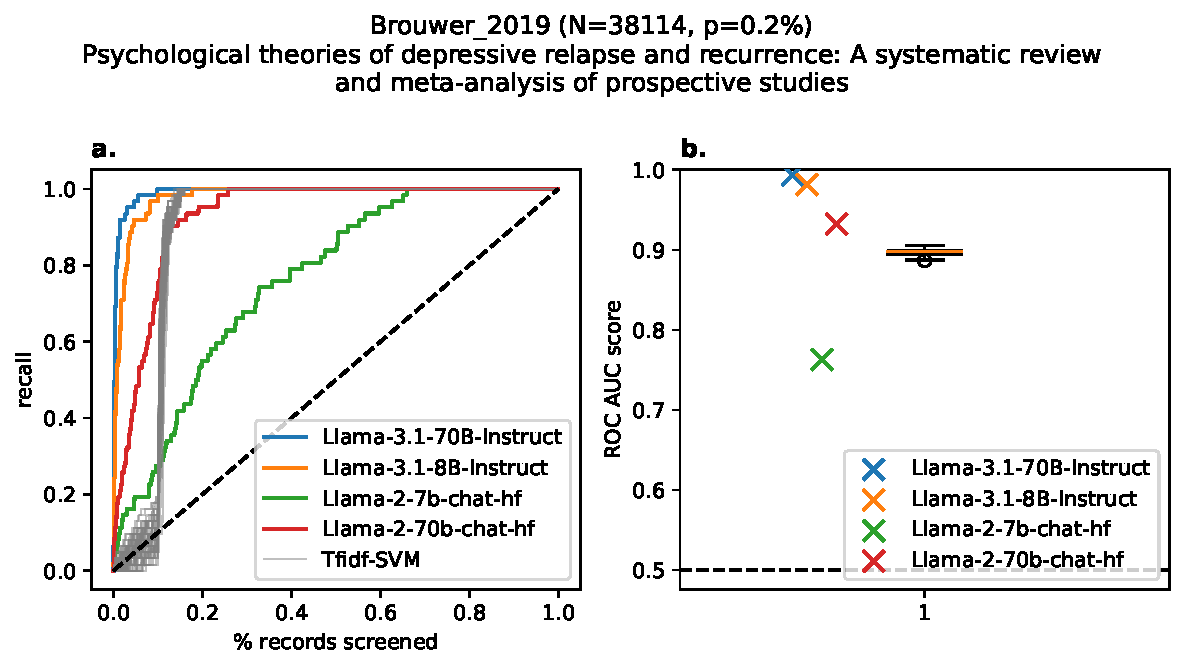
\includegraphics[width=\linewidth]{../../figures/Brouwer_2019.pdf}
		\caption{Rankings produced by LLM-assisted screening (coloured lines) and by active learning using a support vector machine. Left panel shows the recall achieved at different proportions of relevant documents screened. Right panel shows the distribution of ROC AUC scores for the support vector machine approach (boxplot) and for LLMs (coloured crosses)}
		\label{fig:rankings}
	\end{figure}
	
	First, we start by examining the rankings produced by our ML-assisted screening processes. Figure \ref{fig:rankings} shows these for a selected review dataset on Psychological theories of depressive relapse and recurrence, which contained 38,114 records, of which 0.2\% were relevant. Looking at the left side, we see that all evaluated models result in the identification of all relevant documents before all documents have been screened, meaning that work savings are in principle possible. On the right-hand side, we see the Receiver Operating Characteristic - Area Under the Curve (ROC-AUC) score, which measures the likelihood that a random relevant document is ranked higher than a random irrelevant record. A score of 1 indicates that all relevant documents are correctly identified first, before any irrelevant documents have been seen. A score of 0.5 indicates that the ranking is no better than chance.
	

\begin{figure}
	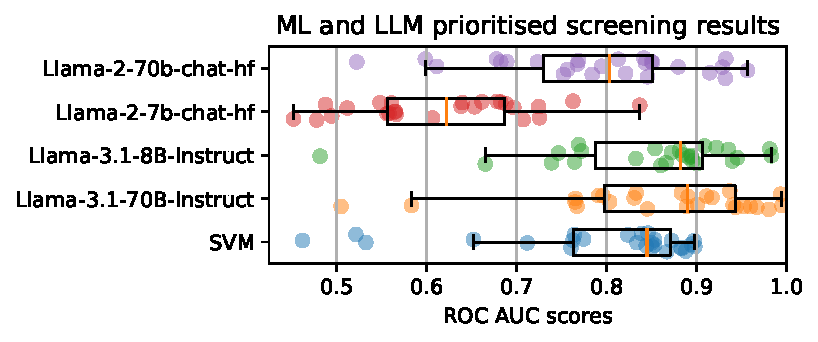
\includegraphics[width=\columnwidth]{../../figures/macro_comparison.pdf}
	\caption{The distribution of ROC AUC scores across datasets. The results for the support vector machine (SVM) display the median score for each dataset.}
	\label{fig:macro}
\end{figure}

\begin{table}
	\centering
	\begin{tabular}{llrrrrr}
\toprule
 & model & SVM & Llama-2-7b & Llama-2-70b & Llama-3.1-8B & Llama-3.1-70B \\
r target & confidence &  &  &  &  &  \\
\midrule
0.80 & 0.50 & 0.938 & \textbf{0.758} & 0.893 & 0.911 & 0.911 \\
 & 0.80 & 0.924 & \textbf{0.797} & 0.866 & 0.845 & 0.889 \\
 & 0.90 & 0.900 & 0.818 & 0.872 & 0.836 & 0.876 \\
 & 0.95 & 0.867 & 0.806 & 0.888 & 0.878 & 0.878 \\
 & 0.99 & 0.811 & 0.838 & 0.865 & 0.876 & 0.886 \\
\cline{1-7}
0.90 & 0.50 & 0.963 & 0.905 & 0.936 & 0.957 & 0.954 \\
 & 0.80 & 0.957 & 0.900 & 0.958 & 0.961 & 0.933 \\
 & 0.90 & 0.947 & 0.937 & 0.959 & 0.953 & 0.939 \\
 & 0.95 & 0.933 & 0.943 & 0.944 & 0.947 & 0.939 \\
 & 0.99 & 0.928 & 0.941 & 0.947 & 0.926 & 0.958 \\
\cline{1-7}
0.95 & 0.50 & 0.979 & \textbf{0.947} & 1.000 & 0.981 & 0.987 \\
 & 0.80 & 0.974 & 0.973 & 0.976 & 0.975 & 0.979 \\
 & 0.90 & 0.973 & 0.968 & 0.981 & 0.978 & 0.980 \\
 & 0.95 & 0.964 & 0.973 & 0.982 & 0.976 & 0.968 \\
 & 0.99 & 0.973 & 0.975 & 0.986 & 0.983 & 0.975 \\
\cline{1-7}
0.99 & 0.50 & 1.000 & 1.000 & 1.000 & 1.000 & 1.000 \\
 & 0.80 & 0.994 & 1.000 & 1.000 & 1.000 & 0.991 \\
 & 0.90 & 0.993 & 0.996 & 1.000 & 0.999 & 0.996 \\
 & 0.95 & 0.993 & 0.997 & 1.000 & 0.999 & 0.996 \\
 & 0.99 & 0.996 & 0.992 & 0.999 & 0.997 & 0.996 \\
\cline{1-7}
\bottomrule
\end{tabular}

	\caption{Recall achieved at the 1-confidence percentile across model runs. Values below the recall target are highlighted in bold.}
	\label{tab:recall}
\end{table}

	
	
	Overall, across the X datasets, Llama3.1 models achieves a higher ROC AUC score than the SVM baseline, while Llama2 models achieve a lower score (figure \ref{fig:macro}). Across both generations of Llama models, models with more parameters achieved higher scores than models with fewer paramaters. This difference was more pronounced for Llama2 than for Llama3.1. 
	
	Next, we apply the stopping criteria to all prioritised runs across all model and dataset combinations, and analyse the recall achieved and the work savings that would have been made. In table \ref{tab:recall}, we show the recall achieved at the percentile of model runs given by 1 minus the confidence interval, for each targeted recall level. 
	For example, if we had used SVM and had stopped screening with $p=0.5$ for a recall target of $0.8$, we would have achieved a recall level of at least $0.94$ 50\% of the time. In other words, we would have missed our recall target \textit{less than} 50\% of the time, meaning that our confidence estimation was conservative (in line with expectations from \cite{callaghan_statistical_2020}).
	Moreover, across 100 combinations of recall target, confidence level, and model, the target was only missed more than would be expected given the confidence level in 3 cases (highlighted in bold text). Moreover, for each of these cases the percentiles are highly imprecise, as they are calculated over the distribution of 26 datasets. For the case of SVM, where there are 100 runs for each dataset, the target was never missed more than would have been expected given the confidence level. This highlights that the stopping criteria developed in \cite{callaghan_statistical_2020} provide a highly effective way to quantify and mitigate the risks of missing relevant studies.
	
	\begin{table}
		\centering
		\begin{tabular}{lllllll}
\toprule
 & model & SVM & Llama-2-7b & Llama-2-70b & Llama-3.1-8B & Llama-3.1-70B \\
r target & confidence &  &  &  &  &  \\
\midrule
0.80 & 0.50 & 0.646 (0.13) & 0.459 (0.12) & 0.572 (0.17) & 0.638 (0.12) & \textbf{0.659 (0.15)} \\
 & 0.80 & \textbf{0.531 (0.17)} & 0.286 (0.12) & 0.437 (0.17) & 0.527 (0.14) & 0.523 (0.16) \\
 & 0.90 & \textbf{0.477 (0.17)} & 0.230 (0.10) & 0.379 (0.17) & 0.475 (0.16) & 0.472 (0.17) \\
 & 0.95 & \textbf{0.433 (0.17)} & 0.205 (0.08) & 0.336 (0.16) & 0.408 (0.17) & 0.428 (0.17) \\
 & 0.99 & \textbf{0.364 (0.17)} & 0.159 (0.07) & 0.263 (0.15) & 0.340 (0.17) & 0.342 (0.16) \\
\cline{1-7}
0.90 & 0.50 & \textbf{0.552 (0.15)} & 0.291 (0.13) & 0.454 (0.17) & 0.534 (0.15) & 0.529 (0.17) \\
 & 0.80 & \textbf{0.411 (0.17)} & 0.183 (0.07) & 0.299 (0.17) & 0.375 (0.17) & 0.388 (0.18) \\
 & 0.90 & \textbf{0.350 (0.16)} & 0.134 (0.07) & 0.241 (0.14) & 0.327 (0.17) & 0.320 (0.17) \\
 & 0.95 & \textbf{0.294 (0.17)} & 0.110 (0.07) & 0.208 (0.14) & 0.272 (0.16) & 0.268 (0.17) \\
 & 0.99 & \textbf{0.224 (0.16)} & 0.076 (0.06) & 0.156 (0.13) & 0.202 (0.14) & 0.198 (0.15) \\
\cline{1-7}
0.95 & 0.50 & \textbf{0.441 (0.16)} & 0.197 (0.08) & 0.330 (0.16) & 0.403 (0.18) & 0.427 (0.18) \\
 & 0.80 & \textbf{0.283 (0.17)} & 0.100 (0.07) & 0.201 (0.14) & 0.254 (0.15) & 0.256 (0.16) \\
 & 0.90 & \textbf{0.225 (0.16)} & 0.073 (0.07) & 0.154 (0.12) & 0.197 (0.14) & 0.198 (0.15) \\
 & 0.95 & \textbf{0.181 (0.15)} & 0.056 (0.06) & 0.121 (0.11) & 0.157 (0.13) & 0.158 (0.14) \\
 & 0.99 & \textbf{0.118 (0.12)} & 0.035 (0.04) & 0.079 (0.08) & 0.102 (0.10) & 0.100 (0.11) \\
\cline{1-7}
0.99 & 0.50 & \textbf{0.288 (0.14)} & 0.104 (0.08) & 0.207 (0.13) & 0.249 (0.13) & 0.264 (0.15) \\
 & 0.80 & 0.113 (0.09) & 0.042 (0.04) & 0.082 (0.07) & 0.100 (0.08) & \textbf{0.117 (0.09)} \\
 & 0.90 & 0.060 (0.06) & 0.022 (0.02) & 0.046 (0.05) & 0.052 (0.05) & \textbf{0.064 (0.06)} \\
 & 0.95 & \textbf{0.038 (0.05)} & 0.013 (0.02) & 0.027 (0.04) & 0.031 (0.04) & 0.038 (0.04) \\
 & 0.99 & \textbf{0.016 (0.03)} & 0.005 (0.01) & 0.011 (0.02) & 0.012 (0.02) & 0.015 (0.03) \\
\cline{1-7}
\bottomrule
\end{tabular}

		\caption{Average proportional work savings across datasets for each combination of  model recall target and confidence level. For the SVM column where there are multiple runs per dataset, we first calculate the median value for each dataset before aggregating across datasets.}
		\label{tab:wssp}
	\end{table}
	
	We now turn to the work savings that would have been achieved at the stopping points given by the stopping criteria. Table \ref{tab:wssp} shows the mean and standard deviation of the work savings achieved for each combination of model, recall target, and confidence level. For low recall targets and low levels of confidence, large work savings are possible (>50\%). Increasing either the recall target or the level of confidence reduces the work savings that can be achieved. For example, for a recall target of 99\%, it is still possible to achieve work savings of 28.8\%, as long as one accepts a 50-50 chance of missing the target. However, if one wants to be 99\% confident that a 99\% recall target has not been missed, on average one would only save 1.6\% of the work.
	
	\begin{table}
		\centering
		\begin{tabular}{llrrrrr}
\toprule
 & model & SVM & Llama-2-7b & Llama-2-70b & Llama-3.1-8B & Llama-3.1-70B \\
r target & confidence &  &  &  &  &  \\
\midrule
0.80 & 0.50 & 126,898 & 100,248 & 121,777 & 127,401 & \textbf{132,808} \\
 & 0.80 & 113,708 & 64,568 & 97,147 & 111,411 & \textbf{114,748} \\
 & 0.90 & 105,053 & 57,678 & 90,327 & 101,871 & \textbf{106,668} \\
 & 0.95 & 98,503 & 48,608 & 83,338 & 94,921 & \textbf{101,288} \\
 & 0.99 & \textbf{87,803} & 37,838 & 71,397 & 79,471 & 85,058 \\
\cline{1-7}
0.90 & 0.50 & 114,988 & 65,778 & 99,217 & 112,011 & \textbf{115,498} \\
 & 0.80 & 93,923 & 42,768 & 79,807 & 83,661 & \textbf{97,438} \\
 & 0.90 & \textbf{84,658} & 34,158 & 65,007 & 76,701 & 82,268 \\
 & 0.95 & \textbf{76,483} & 28,748 & 59,447 & 69,251 & 73,108 \\
 & 0.99 & \textbf{62,350} & 23,118 & 49,790 & 55,091 & 59,088 \\
\cline{1-7}
0.95 & 0.50 & 98,258 & 44,408 & 82,907 & 94,731 & \textbf{101,318} \\
 & 0.80 & \textbf{74,098} & 27,238 & 58,587 & 64,281 & 68,678 \\
 & 0.90 & \textbf{63,245} & 21,738 & 44,470 & 53,091 & 57,388 \\
 & 0.95 & \textbf{54,860} & 18,781 & 37,370 & 45,954 & 48,671 \\
 & 0.99 & \textbf{41,676} & 13,545 & 27,171 & 34,855 & 35,592 \\
\cline{1-7}
0.99 & 0.50 & \textbf{63,573} & 22,638 & 42,897 & 54,811 & 55,378 \\
 & 0.80 & \textbf{31,323} & 11,158 & 20,597 & 29,191 & 30,398 \\
 & 0.90 & \textbf{21,160} & 5,825 & 13,480 & 13,641 & 18,478 \\
 & 0.95 & \textbf{16,229} & 4,065 & 8,837 & 9,435 & 11,938 \\
 & 0.99 & \textbf{7,980} & 1,985 & 4,355 & 4,934 & 6,625 \\
\cline{1-7}
\bottomrule
\end{tabular}

		\caption{Average proportional work savings across datasets for each combination of  model recall target and confidence level. For the SVM column where there are multiple runs per dataset, we first calculate the median value for each dataset before aggregating across datasets.}
		\label{tab:wsst}
	\end{table}
	
	Despite the previous results showing that the largest and newest LLMs achieved superior ROC-AUC scores to a simpler SVM model with iterative retraining, once we look at the work savings that would have been achieved in a realistic setting, we see that in the vast majority of settings, we would still save more work with a simpler SVM model. For 17 of the 20 combinations of recall targets and confidence levels shown in table \ref{tab:wssp}, the highest work savings (highlighted in bold) are achieved with an SVM.
	
	Finally, we look at total work savings available across datasets (table \ref{tab:wsst}). The Synergy dataset contains systematic review datasets that range from 258 to 48,375 records. 
%	Because of the relationship between the number of records that have been seen and the confidence intervals calculated as part of the stopping criterion, larger proportional work savings are in principle possible with larger datasets \cite{callaghan_statistical_2020}. 
	Screening each of the datasets by hand would have required 169,288 records to be screened.	
	If we had aimed for a recall target of 80\% and accepted a 50\% chance of missing the target, this number could have been reduced by 100,248 in the worst performing model (Llama 2 7b) to 132,808 in the best performing model (Llama 3.1 70b).
	Again, increasingly ambitious recall targets and increasingly high levels of confidence reduce the amount of work that can be saved substantially. It is still possible to achieve an ambitious recall target of 90\% with 90\% confidence and save almost half of the otherwise required work (63,245 records). However, in highly ambitious settings, such as 99\% recall with 99\% confidence, only minimal work savings are possible (7,980 records, or just under 5\%)

	
	\section*{Discussion}
	
	These results add to previous evidence that it is possible to \textit{safely} use prioritised screening approaches that can guarantee a given level of recall with a given level of confidence \cite{callaghan_statistical_2020}. Across a wide range of datasets, as well as a wide range of different models, the stopping criteria ensured that the targeted level of recall was missed no more than expected given the confidence level.
	
	Next, we add to promising evidence that LLMs can produce remarkably good rankings of abstracts for screening, even with very little human input. However, when we consider a practical use-case, the benefits of using LLMs for screening seem to be much more limited. In the majority of settings, higher work savings are achieved with much simpler SVM models.
	
	Simplified version, no inclusion criteria - but also simplified SVM setting, no parameter tuning, large batches, no finetuned.
	
	Possibility to combine
	
	Scientific treatment of the costs and benefits of different options. 
	
	
	
	\bibliographystyle{unsrt}
	
	\bibliography{LLMs/stopping-criteria}
	%\bibliography{../LLMs}
	
	\appendix
	
	\section*{Supplementary Material}
	
	\subsection*{Prompt template}
	
	
\end{document}